\subsection{Results}
\label{sec:results}

\begin{table}[t]
\centering
\caption{Comparison with other methods on CrossTask dataset.}
\vspace{-3mm}
\scalebox{0.92}{
\begin{tabular}{lccccccccc}
\toprule
& \multicolumn{3}{c}{$T$ = 3} & & \multicolumn{3}{c}{$T$ = 4} & $T$=5 & $T$ = 6 \\ 
\cline{2-4} \cline{6-8}
{Models}           & SR$\uparrow$    & mAcc$\uparrow$   & mIoU$\uparrow$  &   & SR$\uparrow$    & mAcc$\uparrow$   & mIoU$\uparrow$  & SR$\uparrow$ & SR$\uparrow$ \\ \midrule
{Random} &   $<$0.01    &    0.94    &   \color{gray}1.66    &   &   $<$0.01    &    0.83    &   \color{gray}1.66   & $<$0.01 & $<$0.01  \\
{Retrieval-Based}   &   8.05    &   23.30     &   \color{gray}32.06    &   &   3.95    &    22.22    &    \color{gray}36.97   & 2.40 & 1.10  \\
{WLTDO}            &   1.87    &    21.64    &   \color{gray}31.70   &    &   0.77    &    17.92    &    \color{gray}26.43  & --- & ---  \\
{UAAA}             &   2.15    &   20.21     &   \color{gray}30.87   &    &   0.98    &   19.86     &  \color{gray}27.09   & --- & ---   \\
{UPN}               &   2.89    &    24.39    &   \color{gray}31.56     &  &   1.19    &   21.59     &   \color{gray}27.85   & --- & ---  \\
{DDN}              &   12.18    &    31.29    &    \color{gray}47.48    &  &   5.97    &    27.10    &    \color{gray}48.46  & 3.10 & 1.20  \\
{PlaTe}              &   16.00    &    36.17    &    \color{gray}65.91   &   &   14.00    &    35.29    &    \color{gray}55.36   & --- & --- \\
{Ext-GAIL}         &   21.27    &   49.46     &   \color{gray}61.70    &   &   16.41    &    43.05    &   \color{gray}60.93   & --- & ---  \\
{P$^3$IV}             &   23.34    &   49.96     &   \color{gray}73.89   &    &   13.40    &   44.16     &   \color{gray}70.01  & 7.21 & 4.40   \\
{EGPP}             & 26.40 & 53.02 & \color{gray}\underline{74.05} & & 16.49 & 48.00 & \color{gray}\underline{70.16} & 8.96 & 5.76 \\
{PDPP$\dagger$ }             &   37.2 & 64.67 &  66.57  &  &  21.48 &  57.82 &  65.13 &  13.45 &  8.41 \\
{KEPP$\dagger$ }             &   38.12 & \underline{64.74} &  \underline{67.15}  &  &  24.15 &  \underline{59.05} &  \underline{66.64} &  14.20 &  9.27 \\
{SCHEMA$\dagger$}             &   \underline{38.93} & 63.80 & \bf \color{gray}79.82 &  &  \underline{24.50} &  58.48 &  \bf \color{gray}76.48 &  \underline{14.75} & \bf  10.53 \\
\midrule
{MTID (Ours)$\dagger$}             &   \bf 40.45 & \bf 67.19 & \bf 69.17  &  & \bf 24.76 & \bf 60.69 &  \bf 67.67 & \bf 15.26 & \underline{10.30} \\
\bottomrule
\end{tabular}
}

\label{tab:crosstask}
\end{table}


\begin{table}
\centering
\caption{Classification results on all datasets.}
\scalebox{0.92}{
\begin{tabular}{l c c c c c c c c c c}
\toprule
   & \multicolumn{4}{c}{CrossTask$_{How}$} &  & \multicolumn{2}{c}{COIN} & 
 & \multicolumn{2}{c}{NIV} \\ 
\cline{2-5} \cline{7-8} \cline{10-11}
Models  & $T$ = 3 & $T$ = 4 & $T$ = 5 & $T$ = 6 & 
 &$T$ = 3 & $T$ = 4 & &$T$ = 3 & $T$ = 4 \\ \midrule
PDPP & 92.43 & 92.98 & 93.39 & 93.20 &  & 79.42 & 79.42& & 100.00 & 100.00 \\ 
MTID (Ours) & \bf 93.67 & \bf 94.03 & \bf 94.02 & \bf 94.26 &  & \bf 81.47 & \bf 81.47& & \bf 100.00 & \bf 100.00 \\ 
\bottomrule
\end{tabular}
}
\label{tab:classifier}
\vspace{-0.3cm}
\end{table}
 



\begin{table}[htbp]
\centering
\caption{Comparisons on COIN and NIV datasets.}
\scalebox{0.83}{
\begin{tabular}{>{\arraybackslash}p{2cm} cc c cc >{\arraybackslash}p{2cm} cc c cc}
\toprule
& \multicolumn{2}{c}{$T$ = 3} & & \multicolumn{2}{c}{$T$ = 4} &
& \multicolumn{2}{c}{$T$ = 3} & & \multicolumn{2}{c}{$T$ = 4} \\ 
\cline{2-3} \cline{5-6} \cline{8-9} \cline{11-12}
{Models(COIN)}  & SR$\uparrow$    & mAcc$\uparrow$   &   & SR$\uparrow$    & mAcc$\uparrow$ &
{Models(NIV)}   & SR$\uparrow$    & mAcc$\uparrow$   &   & SR$\uparrow$    & mAcc$\uparrow$ \\ 
\midrule
Random       & $<$0.01    & $<$0.01    &  & $<$0.01    & $<$0.01    &
Random       & 2.21       & 4.07       &  & 1.12       & 2.73       \\
DDN          & 13.90      & 20.19      &  & 11.13      & 17.71      &
DDN          & 18.41      & 32.54      &  & 15.97      & 27.09      \\
P$^3$IV      & 15.40      & 21.67      &  & 11.32      & 18.85      &
Ext-GAIL     & 22.11      & 42.20      &  & 19.91      & 36.31      \\
EGPP         & 19.57      & 31.42      &  & 13.59      & 26.72      &
P$^3$IV      & 24.68      & \underline{49.01} &  & 20.14 & 38.36    \\
PDPP         & 21.33      & 45.62      &  & 14.41      & 44.10      &
EGPP         & 26.05      & \bf 51.24  &  & 21.37      & \underline{41.96} \\
KEPP         & 20.25      & 39.87      &  & 15.63      & 39.53      &
KEPP         & 24.44      & 43.46      &  & 22.71      & 41.59      \\
SCHEMA       & \bf 32.09  & \underline{49.84} &  & \underline{22.02} & \underline{45.33} &
SCHEMA       & \underline{27.93} & 41.64 &  & \underline{23.26} & 39.93 \\
\midrule
MTID (Ours)  & \underline{30.90} & \bf 52.17 &  & \bf 23.10 & \bf 49.71 &
MTID (Ours)  & \bf 29.63 & 48.02 &  & \bf 25.76 & \bf 46.62 \\
\bottomrule
\end{tabular}
}
\label{tab:combined}
\end{table}

\textbf{Results for Task Classifier.} The first stage of our approach involves predicting the task class based on the given start and goal observations. We implement this using transformer models, replacing the two-layer Res-MLP architecture employed in \citet{wang2023pdpp}, and train it using a simple cross-entropy (CE) loss. The classification results are presented in \Cref{tab:classifier}. Our method consistently outperforms previous approaches in all evaluated aspects.


\textbf{Comparisons on CrossTask.} We evaluate performance on CrossTask using four prediction horizons, with the results shown in \Cref{tab:crosstask}. 
% It is important to note that we compute the mIoU by averaging the IoU values for each action sequence individually, rather than over a mini-batch, which may result in lower mIoU values compared to mini-batch calculations. 
The results in \Cref{tab:crosstask} demonstrate that our method outperforms all other approaches across all metrics, except for the SR at $T = 6$, where our model ranks second. These improvements are consistent across longer prediction horizons ($T = 4, 5, 6$) and other step-level metrics, including mAcc and mIoU.


\textbf{Comparisons on NIV and COIN.} \Cref{tab:combined} presents our evaluation results on the NIV and COIN datasets, demonstrating that our approach consistently outperforms or matches the best-performing methods across both datasets. 
% Specifically, on the NIV dataset, where both SR and mAcc are relatively high, our model improves SR by more than 2\% for both horizons and surpasses the previous best mAcc by over 7\%. For the larger COIN dataset, where SR improves by more than 1\% at $T=4$, our model achieves a significant improvement of more than 4\% in mAcc. 
These results highlight that our model performs robustly across datasets of varying sizes.




\subsection{Ablation Studies} 


\begin{wraptable}{r}{0.5\textwidth}
\vspace{-14pt}
\centering
\caption{Ablation studies on our loss function. Note: W: Weights on Both Sides, GW: Gradient Weights, M: Mask.}
\label{tab:loss_ablation}
\scalebox{0.87}{
\begin{tabular}{@{}*{6}{>{\centering\arraybackslash}m{0.06\textwidth}}@{}}
\toprule
ID & MSE & W & GW & M & SR$\uparrow$ \\ 
\midrule
1 & \checkmark &  &  &  & 11.89 \\
2 & \checkmark & \checkmark &  &  & 13.90 \\
3 & \checkmark &  & \checkmark &  & \underline{15.10} \\
4 & \checkmark &  &  & \checkmark & 13.26 \\
5 & \checkmark & \checkmark &  & \checkmark & 13.93 \\
6 & \checkmark &  & \checkmark & \checkmark & \textbf{15.26} \\
\bottomrule
\end{tabular}
}
\vspace{-9pt}
\end{wraptable}
\textbf{Task-Adaptive Masked Proximity Loss.}~\Cref{tab:loss_ablation} demonstrates the effectiveness of our proposed loss strategy with $T=5$ on the CrossTask dataset, using Mean Squared Error (MSE) as the base loss. The results show that both the task-adaptive mask and gradient weights improve performance. While MSE alone results in lower scores, adding masks and fixed weights provides moderate improvement. Our approach, which incorporates gradient-weighted loss and intermediate supervision, significantly boosts performance by leveraging richer task-relevant features. 


\begin{wraptable}{r}{0.5\textwidth}
\vspace{-10pt}
\centering
\caption{Ablation study on projection and phase when $T=3$ on CrossTask dataset. Note: ``CP'' denotes the condition projection. }
\label{tab:MP}
\scalebox{0.85}{
\begin{tabular}{@{}l*{3}{>{\centering\arraybackslash}m{0.09\textwidth}}@{}}
\toprule
{Models}          & SR$\uparrow$ & mAcc$\uparrow$   & mIoU$\uparrow$  \\ \midrule
{CP on both}        &   \underline{39.17} & \underline{66.49} & \underline{68.38}  \\
{MP on iteration}          & 3.38 & 10.17 & 9.66 \\
{MP on initialization} & \textbf{40.45} & \textbf{67.19} & \textbf{69.17}\\
\bottomrule
\end{tabular}
}
\vspace{-10pt}
\end{wraptable}
\textbf{Masked Projection.} \Cref{tab:MP} demonstrates that our masked projection (MP) on $\hat{x}_N$ as input to the U-Net enhances performance by filtering out irrelevant actions, allowing the model to focus on task-relevant actions. We also experimented with applying the mask during iterations, but this approach proved ineffective. During the denoising process, the input matrix contains both positive and negative logits, and in some cases, negative values can improve the final score. Masking at this stage disrupted the natural behavior of the logits and the diffusion denoising process. Furthermore, applying the mask before the condition projection led to sub-optimal results due to inaccurate task labels. Therefore, we apply the mask only after the condition projection for optimal performance.



\begin{figure}[h]
% \vspace{-4mm}
\centering
\subfloat[Ablation studies on different simple initialization methods.]{%
    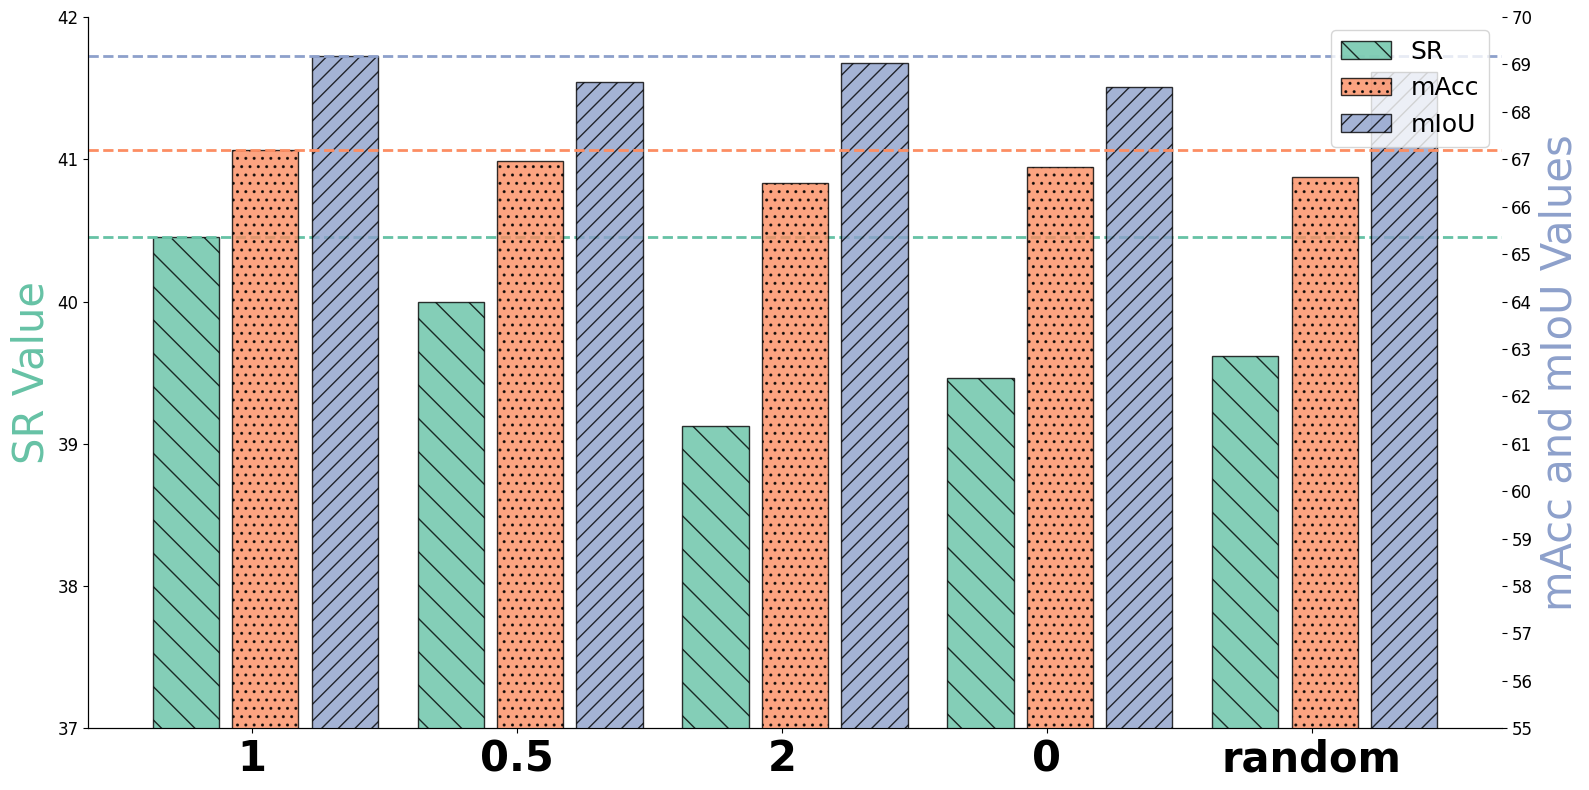
\includegraphics[width=0.45\textwidth]{figures/int1.png}
    \label{fig:int1}
}
\hfill
\subfloat[Ablation studies on different return values.]{%
    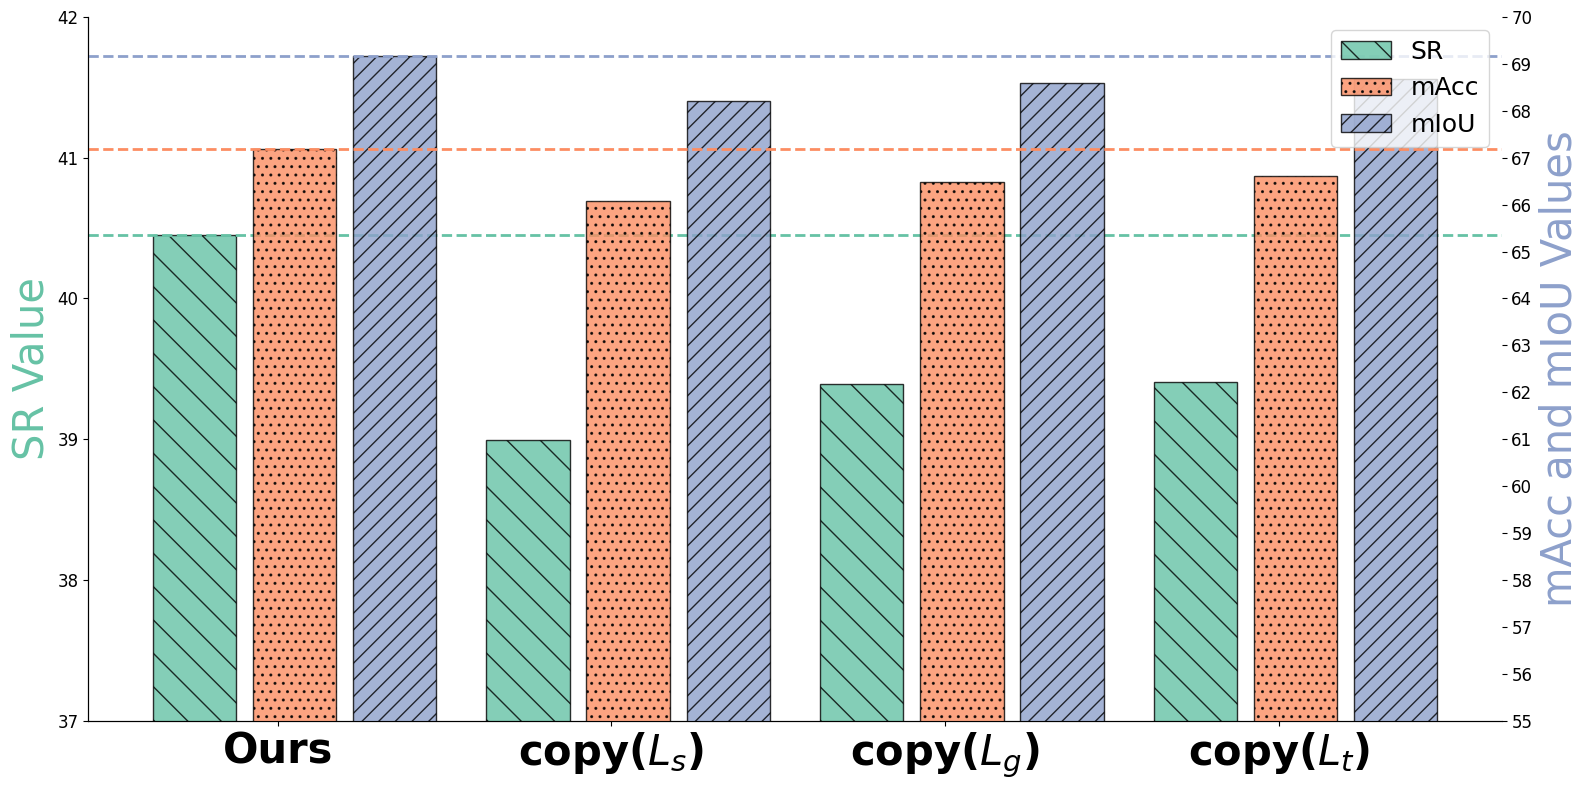
\includegraphics[width=0.45\textwidth]{figures/int2.png}
    \label{fig:int2}
}
\vfill
\subfloat[Ablation studies on selection with different interpolated features.]{
    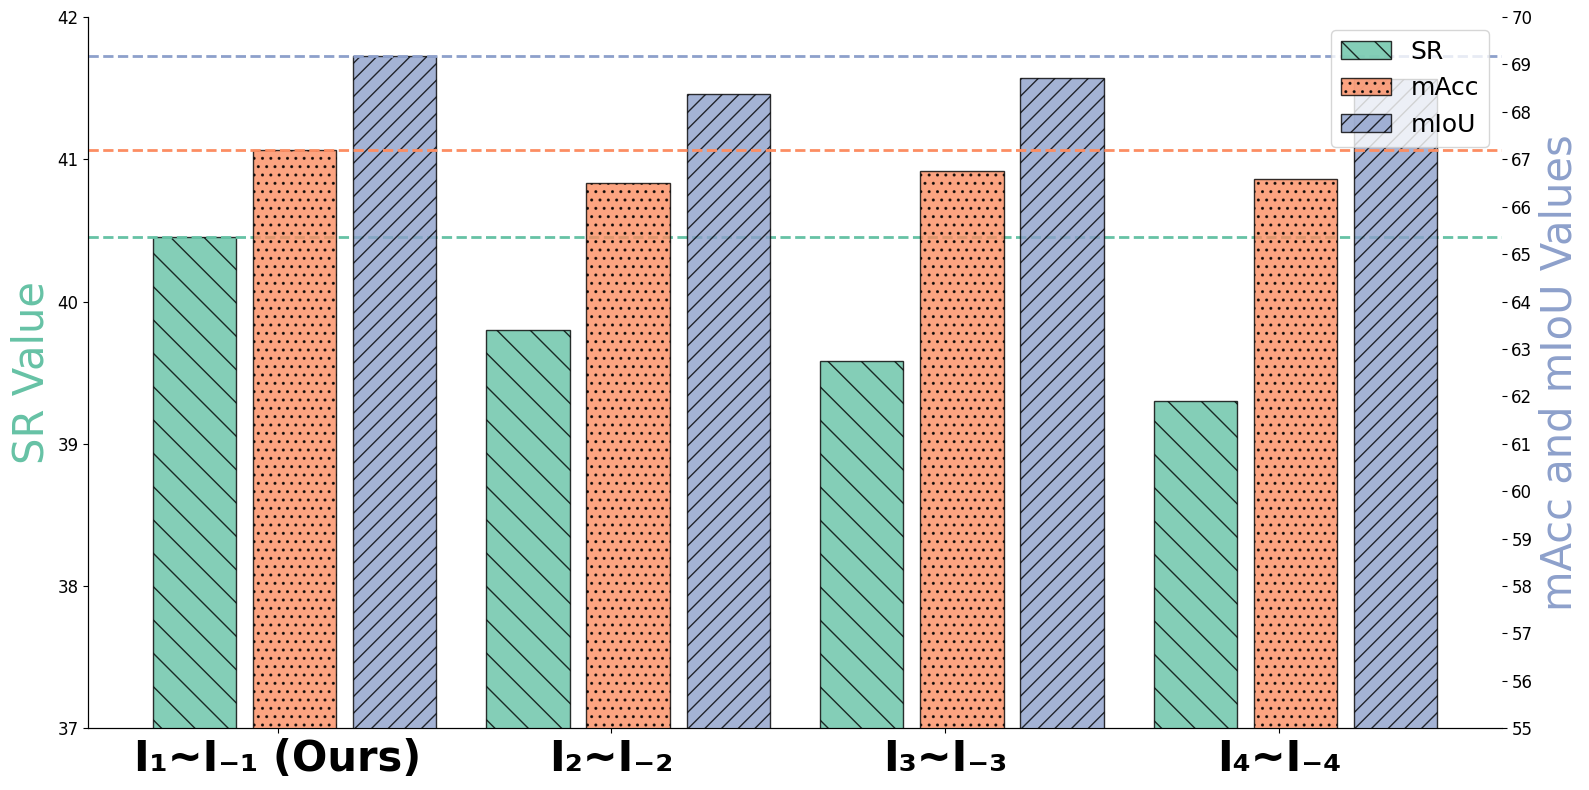
\includegraphics[width=0.45\textwidth]{figures/int3.png}
    \label{fig:int3}
}
\hfill
\subfloat[Ablation studies on different fusion methods.]{%
    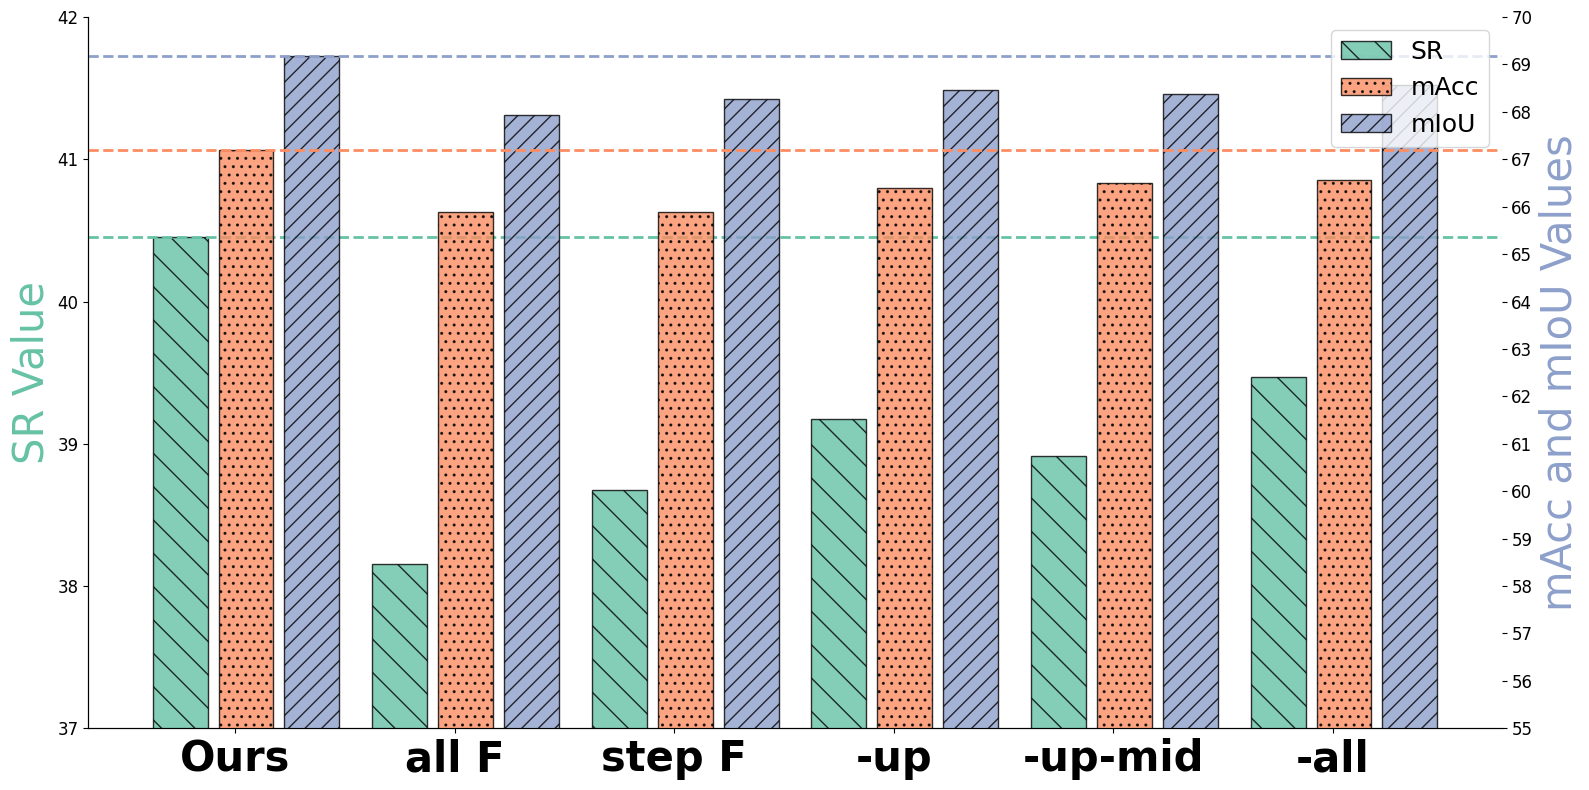
\includegraphics[width=0.45\textwidth]{figures/int4.png}
    \label{fig:int4}
}
\caption{Ablation Studies for Interpolation Strategy. \Cref{fig:int1} shows different initialization coefficient values $\tau$; \Cref{fig:int2} illustrates the features generated by the interpolator, where ``$copy(L_g)$'' means $I_j = L_g$, and ``$copy(L_t)$'' indicates $I_j = L_s$ for $j \leq \frac{M}{2}$ and $I_j = L_g$ for $j > \frac{M}{2}$. In \Cref{fig:int3}, $I_i$ to $I_{-i}$ indicates that we use interpolated features from the $i$-th to the last $i$-th for the second interpolation. In \Cref{fig:int4}, ``all F'' denotes that each cross-attention module receives $F_{1:M}$ as input, ``step F'' means we input one $F_{\frac{M}{2}}$ at the start and gradually increase the number of features inputted towards both sides, and ``-all'' indicates that we omit inputting $F_j$ during the upsampling, middle-sampling, and downsampling processes in U-Net. }
\label{fig:four_images2}
\end{figure}




% 加上ablation for 100%的结果,展示出分类器仍有不足。





% Following \citet{wang2023pdpp}, we enhance the diffusion model by incorporating a mask during the noise generation process, focusing on the $CrossTask_{How}$ dataset due to its high planning uncertainty.

\begin{wraptable}{r}{0.55\textwidth}
\vspace{-10pt}
\centering
\caption{Component ablation. Note: Int: Interpolation, Enc: Encoder, Trans: Transformer.}
\label{tab:component_ablation}
\scalebox{0.8}{
\begin{tabular}{@{}*{7}{>{\centering\arraybackslash}m{0.07\textwidth}}@{}}
\toprule
ID & Int & Enc & Trans & SR$\uparrow$ & mAcc$\uparrow$ & mIoU$\uparrow$ \\ 
\midrule
1 & \checkmark &  &  & 37.86 & 65.42 & 67.32 \\
2 & \checkmark & \checkmark &  & 39.23 & 66.62 & 68.44 \\
3 & \checkmark &  & \checkmark & \underline{39.49} & \underline{66.81} & \underline{68.68} \\
4 & \checkmark & \checkmark & \checkmark & \textbf{40.45} & \textbf{67.19} & \textbf{69.17} \\
\bottomrule
\end{tabular}
}
\vspace{-10pt}
\end{wraptable}
\textbf{Latent Space Temporal Interpolation Module.} To evaluate the impact of various components within the module, we conduct ablation studies on the CrossTask dataset with $T=3$. \Cref{tab:component_ablation} presents the results. The findings indicate that the observation encoder effectively transforms visual observations into latent features, enhancing causal inference and capturing temporal logic. The interpolator enriches these features by generating multiple interpolated versions, which aids in reasoning. The transformer encoder further refines these features, ensuring both mathematical interpolation and logical consistency, thereby improving the model's inference capabilities.


\textbf{Interpolation Strategy.} \Cref{fig:four_images2} illustrates our adapted interpolation strategies for contrast. 
Initially, we test different initialization $\tau$ values in \Cref{fig:int1}. The highest score occurs when $\phi$ is initialized to 1, which proves to be the most stable and achieves the best overall performance, indicating that $\phi$ converges close to 1. 
Further experiments in \Cref{fig:int2} compare the use of $L_s$, $L_g$, or a combination of both through copying and direct return. The results show that directly returning $L_g$ performs well, suggesting that $V_g$ may play a critical role in action sequence inference. Although $L_s$ and $L_g$ are unadjusted features, the transformer encoder blocks can refine them to capture richer temporal logic and filter out irrelevant details, resulting in relatively reasonable scores. 
Additionally, we perform a second interpolation using the obtained $F_j$ (\Cref{fig:int3}). This experiment shows that as the features shift towards the center (from $F_i$ to $F_{-i}$), performance declines due to the loss of original information, aligning with our intuition. 
In \Cref{fig:int4}, we examine different fusion strategies for cross-attention. The ``all F'' approach results in sub-optimal performance, potentially due to the inclusion of numerous features being limited by the capacity of the layers, which diminishes the amount of information each feature can carry and introduces disorder. Similarly, the ``step F'' strategy may suffer from the same issue. When cross-attention is removed from various stages of the U-Net, we observe that the more layers are removed, the worse the results become. However, when all layers are removed, the results improve slightly, suggesting that introducing latent features into the U-Net without sufficient information disturbs the original distribution, leading to sub-optimal outcomes.



\subsection{Uncertainty Modeling} 
We present the uncertainty modeling results for CrossTask and NIV in \Cref{tab:combined_uncertainxx}. Two baselines from \citet{wang2023pdpp} are used for comparison: the $Noise$ baseline, which samples from random noise and uses the given observations and task class condition to obtain results in a single step without the diffusion process, and the $Deterministic$ baseline, where $\hat{x}_N=0$ and the model predicts a fixed outcome. We evaluate performance using $KL$ $divergence$, $NLL$, $ModeRec$, and $ModePrec$, as outlined in \citet{zhao2022p3iv}.

Our approach outperforms the baselines on CrossTask, particularly in modeling uncertainty and generating diverse plans. Compared to \citet{wang2023pdpp}, our model excels in the deterministic setting with $T=3$, demonstrating its ability to capture latent temporal relationships even with fewer time steps. For the NIV dataset, we observe that despite its small size, our diffusion-based process still delivers improvements. Additional visualizations are provided in the appendix.


\begin{table}[htbp]
% \vspace{-4mm}
\centering
\caption{The results of uncertain modeling on the CrossTask and NIV datasets.}
\scalebox{0.92}{
\begin{tabular}{l l cccc c cc}
\toprule
& & \multicolumn{4}{c}{CrossTask} & & \multicolumn{2}{c}{NIV} \\
\cline{3-6} \cline{8-9}
Metric & Method & $T=3$ & $T=4$ & $T=5$ & $T=6$ & & $T=3$ & $T=4$ \\
\midrule
\multirow{3}*{KL-Div $\downarrow$}
& Deterministic & 3.12 & 3.88 & 4.39 & \underline{4.04} & & 5.40 & \bf 5.29 \\
& Noise & \underline{2.75} & \underline{3.16} & \underline{4.37} & 4.74 & & \underline{5.36} & 6.03 \\
& Ours & \bf 2.66 & \bf 2.81 & \bf 2.12 & \bf 1.97 & & \bf 4.65 & \underline{5.47} \\
\midrule
\multirow{3}*{NLL $\downarrow$}
& Deterministic & 3.70 & 4.45 & 4.98 & 5.34 & & 5.48 & \bf 5.42 \\
& Noise & \underline{3.33} & \underline{4.04} & \underline{4.95} & \underline{5.32} & & \underline{5.44} & 6.12 \\
& Ours & \bf 3.24 & \bf 3.69 & \bf 3.22 & \bf 3.27 & & \bf 4.74 & \underline{5.56} \\
\midrule
\multirow{3}*{ModePrec $\uparrow$}
& Deterministic & 52.76 & 41.13 & \underline{31.46} & 18.65 & & \underline{27.77} & 26.48 \\
& Noise & \underline{54.30} & \underline{46.15} & 22.52 & \underline{19.09} & & 23.19 & \underline{32.39} \\
& Ours & \bf 56.19 & \bf 47.05 & \bf 32.75 & \bf 22.98 & & \bf 30.75 & \bf 35.88 \\
\midrule
\multirow{3}*{ModeRec $\uparrow$}
& Deterministic & 31.71 & 20.55 & 18.70 & 4.63 & & 26.48 & 21.57 \\
& Noise & \underline{43.92} & \underline{22.35} & \underline{21.53} & \underline{17.53} & & \underline{32.39} & \underline{23.75} \\
& Ours & \bf 47.34 & \bf 37.97 & \bf 39.64 & \bf 35.03 & & \bf 35.88 & \bf 29.90 \\
\bottomrule
\end{tabular}
}
\label{tab:combined_uncertainxx}
\end{table}

